\documentclass[journal]{IEEEtran}

\usepackage{amsmath,amssymb,amsfonts,amsthm}
\usepackage{algorithmicx}
\usepackage{algorithm}
\usepackage{algpseudocode}
\usepackage{graphicx}
\usepackage{textcomp}
\usepackage{booktabs}
\usepackage{cite}
\usepackage{url}
\usepackage{hyperref}
\usepackage{microtype}
\usepackage{balance}

\newtheorem{theorem}{Theorem}
\newtheorem{lemma}{Lemma}
\newtheorem{definition}{Definition}

\begin{document}

\title{Counterfactual Flip-Cost Analysis: Quantifying Pairwise Ordering Ambiguity in Precedence-Constrained Security Timelines}

\author{Varun~Dubey and Kamalesh~N%
\thanks{The authors are with the School of Computer Science and Engineering, Vellore Institute of Technology, Chennai 600127, Tamil Nadu, India (e-mail: varun.dubey2024@vitstudent.ac.in, kamalesh.n2024@vitstudent.ac.in).}}

\maketitle

\begin{abstract}
Reconstructing attack timelines from heterogeneous security event logs is frequently undermined by timestamp distortion, including per-core clock skew, network latency, coarse millisecond quantisation, and deliberate anti-forensic timestomping. While domain causality and system provenance establish invariant partial-order constraints represented as a Directed Acyclic Graph (DAG), resolving the full total order requires finding a linear extension that minimizes disagreements with observed timestamps. This corresponds to the Nearest-Neighbour Kendall-Tau Distance problem on posets, which is known to be NP-complete. In this paper, we introduce a \textbf{counterfactual flip-cost framework} to rigorously assess the sensitivity and ambiguity of pairwise ordering decisions in reconstructed timelines. Unlike process-mining techniques that infer trace distributions across historical case libraries, our approach operates on isolated, single-incident investigations without requiring prior execution logs. We formulate the pairwise flip-cost $\Delta(a, b)$ as the marginal reconstruction penalty incurred when forcing a counterfactual inversion between unconstrained events $a$ and $b$ within a budget-bounded best-first search. Theoretically, this corresponds to the log-ratio of extremal Maximum A Posteriori (MAP) realizations under a precedence-conditioned Mallows ranking model. Furthermore, we develop a diversity-aware candidate selection algorithm based on farthest-first traversal over unconstrained event pairs to expose structurally distinct, near-optimal timelines to forensic analysts. We evaluate our framework across diverse graph topologies under both uncorrelated Gaussian jitter and structured multi-source clock-skew models. On benchmark event DAGs, flip-cost sensitivity achieves an AUROC of 0.891 in discriminating true causal order, outperforming timestamp-margin heuristics (AUROC 0.858), while diversity-aware selection doubles candidate variation (from 0.040 to 0.082) with bounded search expansion overhead. Our findings demonstrate that counterfactual flip-cost provides a principled, objective-relative diagnostic for identifying fragile timeline conclusions prior to operational incident response.
\end{abstract}

\begin{IEEEkeywords}
Digital forensics, incident timeline reconstruction, partial orders, linear extensions, counterfactual analysis, Kendall-tau distance, heuristic search, ordering ambiguity.
\end{IEEEkeywords}

\section{Introduction}
\IEEEPARstart{S}{ecurity} event logs generated by enterprise endpoints, firewalls, operating system audit daemons, and cloud infrastructure are the primary forensic foundation for cyber-incident triage, root-cause analysis, and attack scenario reconstruction \cite{Hossain2017, Cheng2024}. During incident response, security analysts must reconstruct an accurate chronological sequence of events---a \emph{timeline}---to establish the adversary's initial vector of compromise, privilege escalation pathway, and data exfiltration timeline.

However, treating recorded timestamps as ground truth is fundamentally hazardous in operational environments. Real-world event streams suffer from pervasive temporal distortions:
\begin{enumerate}
    \item \textbf{Clock Asynchrony \& Skew:} Network Time Protocol (NTP) synchronization drifts, hypervisor virtualization pauses, and hardware-level clock differences introduce substantial jitter across distributed nodes. Even within a single host, unsynchronized per-core hardware counters can produce non-monotonic timestamps. Recent empirical measurements by Kimm et al. \cite{Kimm2026} demonstrate that between 3.0\% and 3.5\% of host audit records are logged out of order purely due to multi-core timestamp drift.
    \item \textbf{Coarse Quantisation:} Standard commercial off-the-shelf (COTS) logging frameworks (such as Windows Event Logs / EVTX and Syslog) frequently record events with millisecond- or second-level granularity, collapsing genuinely sequential operations into identical timestamps.
    \item \textbf{Adversarial Manipulation:} Sophisticated attackers routinely employ anti-forensic techniques such as \emph{timestomping} (deliberately rewriting metadata timestamps in file systems and logs) to disrupt chronological reconstruction \cite{Peisert2007}.
\end{enumerate}

While kernel-level instrumentation utilizing atomic sequence numbers (e.g., modern \texttt{auditd}, \texttt{sysdig}, or eBPF wrappers) can establish total orders within a single kernel stream \cite{Kimm2026}, such instrumentation is unavailable when fusing forensic logs across disparate enterprise hosts, network appliances, or legacy un-instrumented infrastructure.

To reconstruct a valid timeline without trustworthy timestamps, investigators must rely on \textbf{domain causality and system provenance constraints} \cite{Hossain2017, Cheng2024}. A system cannot read a file before that file is created; a child process cannot execute before its parent invokes \texttt{fork()} or \texttt{CreateProcess()}. Such invariant physical and causal dependencies naturally form a Directed Acyclic Graph (DAG) $G = (V, E)$, defining a partially ordered set (poset) of observed events \cite{Pegoraro2020a}. Any admissible historical timeline must be a \textbf{linear extension} (a topological sort) of this partial order.

When the precedence constraints do not fully determine the sequence of all event pairs, the graph admits multiple valid linear extensions. The number of linear extensions can grow exponentially with the number of unconstrained events, a problem shown by Brightwell and Winkler to be $\#\text{P}$-complete \cite{Brightwell1991}. To identify the most plausible timeline, investigators seek a linear extension that minimizes disagreements with the recorded timestamps---formalized as the \textbf{Nearest-Neighbour Kendall-Tau Distance} between a partial order and a total order. Brandenburg et al. \cite{Brandenburg2011} proved that finding such a minimal-inversion linear extension is \textbf{NP-complete}.

\subsection{The Ordering Ambiguity Dilemma}
In practice, forensic tools typically return a single best-scoring timeline (Top-1) obtained via heuristic search or topological sorting with timestamp tie-breaking. However, returning a single linear extension conceals profound operational fragility:
\begin{itemize}
    \item \textbf{False Decisiveness:} If event $a$ and event $b$ are causally independent and their timestamps differ by only 2~ms, an optimizer will place $a$ before $b$. An investigator might build an entire containment theory around $a \prec b$, unaware that reversing them incurs an insignificant cost penalty.
    \item \textbf{Flaws of Heuristic Baselines:} A naive timestamp margin $|\tau(b) - \tau(a)|$ fails to measure true ambiguity. Two events separated by 500~ms might be strictly bound by a transitive causal chain (making reversal impossible), whereas two events separated by 2 seconds might be causally disconnected and easily flipped without disturbing the rest of the sequence.
    \item \textbf{Limitations of Process-Mining Frameworks:} Prior work on resolving partial orders in event logs (e.g., van der Aa et al. \cite{vanderAa2020}, Pegoraro et al. \cite{Pegoraro2020a, Pegoraro2021}) relies on estimating probabilistic distributions over total orders across hundreds or thousands of repeated trace executions in structured business processes. In forensic incident response, this case-base assumption collapses: an Advanced Persistent Threat (APT) attack is a unique, one-off sequence with no historical distribution from which to estimate transition frequencies.
\end{itemize}

\subsection{Our Approach: Counterfactual Flip-Cost Analysis}
To overcome these limitations, this paper proposes an objective-relative, single-incident sensitivity analysis: \textbf{Counterfactual Flip-Cost Analysis}. 

Rather than presenting an investigator with an arbitrary single sequence or an unranked set of alternatives, we evaluate the stability of specific pairwise ordering decisions. For any unconstrained pair $(a, b)$ ordered $a \prec b$ in the baseline optimal timeline $\pi^*$, we ask the counterfactual question:
\begin{quote}
\emph{``What is the minimum additional cost penalty incurred if we strictly force event $b$ to precede event $a$?''}
\end{quote}

By enforcing the counterfactual constraint $pos(b) < pos(a)$ and performing a budget-bounded best-first search on the augmented DAG, we compute the \emph{flip-cost}:
\begin{equation}
\Delta(a, b) = c_{flip}(a, b) - c(\pi^*)
\end{equation}
If $\Delta(a, b) \approx 0$, the decision $a \prec b$ is highly ambiguous and sensitive; the data cannot decisively support this order. Conversely, a large $\Delta(a, b)$ indicates that reversing the pair severely disrupts timestamp consistency or forces cascading inversions across other dependent events.

As we prove in Section~\ref{sec:problem_formulation}, this combinatorial flip-cost has a direct probabilistic interpretation: it represents the \textbf{exact log-ratio of extremal Maximum A Posteriori (MAP) realizations} under a precedence-conditioned Mallows ranking model \cite{Lu2011}.

\subsection{Key Contributions}
The main contributions of this paper are:
\begin{enumerate}
    \item \textbf{Theoretical Formulation \& Grounding:} We formalize timeline ambiguity as a constrained Kendall-tau inversion minimization problem on posets, prove its computational hardness via reduction to the Nearest-Neighbour Kendall-Tau Distance \cite{Brandenburg2011}, and establish its theoretical equivalence to the MAP ratio of a conditioned Mallows model.
    \item \textbf{Counterfactual Flip-Cost Metric:} We define the pairwise flip-cost $\Delta(a, b)$ and present an efficient, budget-bounded best-first search algorithm that computes exact or bounded sensitivity scores with explicit search-exhaustion accounting.
    \item \textbf{Diversity-Aware Candidate Selection:} To avoid returning near-identical candidate timelines, we formulate a farthest-first selection mechanism operating over the space of unconstrained event pairs ($P_{free}$), enabling investigators to inspect structurally diverse, low-cost timelines.
    \item \textbf{Comprehensive Empirical Evaluation:} We benchmark the proposed framework across varied graph topologies under both uncorrelated Gaussian timestamp jitter and structured multi-source clock-skew models. We demonstrate that flip-cost scoring achieves an AUROC of 0.891 in discriminating true causal order against timestamp margins (0.858), evaluate the computational trade-offs of diversity-aware selection, and provide paired bootstrap confidence intervals.
\end{enumerate}

\subsection{Paper Organization}
The remainder of this paper is organized as follows. Section~\ref{sec:related_work} reviews related work in poset linear extensions, process mining under timestamp uncertainty, and provenance-based attack reconstruction. Section~\ref{sec:problem_formulation} formalizes the problem statement, inversion cost objective, computational complexity, and Mallows model derivation. Section~\ref{sec:methodology} details the proposed methodology, including bounded best-first search, counterfactual flip-cost computation, and diversity-aware candidate selection. Section~\ref{sec:experimental_setup} describes the experimental setup, simulation configurations, and evaluation metrics. Section~\ref{sec:results} presents the empirical results, ablation studies, and scalability analysis. Section~\ref{sec:validity} discusses limitations and validity threats. Finally, Section~\ref{sec:conclusion} concludes the paper and highlights avenues for future research.

\section{Related Work}
\label{sec:related_work}

The problem of reconstructing and evaluating event timelines under timestamp uncertainty intersects four active research domains: (i) partial-order resolution in process mining, (ii) combinatorial algorithms for partially ordered sets (posets) and linear extensions, (iii) diverse heuristic search and top-$K$ planning, and (iv) system provenance and digital log forensics.

\subsection{Partial-Order Resolution in Event Logs and Process Mining}
Event ordering under temporal imprecision has been investigated extensively within the process mining community. When recorded timestamps overlap, an execution trace ceases to be a strictly ordered sequence and is naturally generalized to a partial order or Directed Acyclic Graph (DAG) \cite{vanderAa2020, Pegoraro2020a}.

Pegoraro et al. \cite{Pegoraro2020a, Pegoraro2020b} introduced the concept of \emph{behavior graphs} for uncertain event data, where directed edges link events whose timestamp intervals do not overlap. However, behavior graphs represent only admissible constraints; they do not rank the resulting linear extensions or assess the sensitivity of individual ordering decisions.

To resolve ambiguous partial orders for process conformance checking, van der Aa et al. \cite{vanderAa2020} proposed an estimation framework that constructs a probability distribution over the set of total orders consistent with an observed partial order, leveraging behavioral abstractions across large historical event logs. Similarly, Pegoraro et al. \cite{Pegoraro2021} developed probability estimation techniques over uncertain trace realizations. 

\textbf{Critical Distinction:} While these frameworks are effective for recurring business processes where thousands of historical traces are available, they cannot be deployed in \textbf{single-incident cyber forensics}. A security breach or advanced persistent threat (APT) campaign is inherently rare, dynamic, and non-repetitive; an incident responder cannot draw upon a statistical case base of identical prior compromises. Our proposed framework operates purely on a \emph{single-instance} event graph without assuming an underlying process distribution.

\subsection{Combinatorial Complexity of Posets and Linear Extensions}
From a theoretical computer science perspective, an event graph $G = (V, E)$ defines a finite poset $P = (V, \prec)$, and any valid chronological timeline corresponds to a \textbf{linear extension} preserving all relations in $E$.

\begin{itemize}
    \item \textbf{Counting Complexity:} Brightwell and Winkler \cite{Brightwell1991} established that computing the exact number of linear extensions $|\mathcal{L}(G)|$ of an arbitrary poset is $\#\text{P}$-complete. Dittmer and Pak \cite{Dittmer2020} proved that this hardness holds even for posets of height two. While exact dynamic programming algorithms over poset ideals exist (e.g., Kangas et al. \cite{Kangas2016}), they remain exponential in the general case ($O^*(2^n)$).
    \item \textbf{Sampling:} Huber \cite{Huber2006} developed algorithms for exact uniform generation of linear extensions via coupling from the past in expected $O(n^3 \ln n)$ time. However, uniform sampling treats all valid extensions equally, failing to penalize orderings that contradict observed timestamp evidence.
    \item \textbf{Optimal Alignment (Inversion Minimization):} Aligning a linear extension with an observed chronological sequence $\pi_\tau$ requires minimizing the Kendall-tau distance. Brandenburg, Gleißner, and Hofmeier \cite{Brandenburg2011} formalized this as the \emph{Nearest-Neighbour Kendall-Tau Distance between a Partial Order and a Total Order} and proved it to be \textbf{NP-complete}.
    \item \textbf{Precedence-Constrained Ranking:} This problem is closely related to the \emph{Precedence-Constrained Minimum Feedback Arc Set} (FAS) on tournaments \cite{Mastrolilli2011}. Van Zuylen and Williamson \cite{vanZuylen2009} developed deterministic pivoting algorithms and LP relaxations providing constant-factor approximation guarantees for constrained ranking.
\end{itemize}

\subsection{Diverse Top-$K$ Optimization and Heuristic Search}
When multiple near-optimal solutions exist, returning solely the top-1 solution obscures plausible alternative explanations. Classical heuristic search algorithms, such as Eppstein’s algorithm \cite{Eppstein1998} and the $K^*$ algorithm by Aljazzar and Leue \cite{Aljazzar2011}, identify the $K$-shortest paths.

However, in combinatorial permutation problems, top-$K$ search suffers from the \textbf{solution clustering problem}: the top-$K$ linear extensions typically represent trivial local permutations rather than structurally distinct timeline interpretations \cite{Sohrabi2016}. To overcome clustering:
\begin{itemize}
    \item Batra et al. \cite{Batra2012} introduced \emph{Diverse $M$-Best Solutions} for Markov Random Fields, incorporating an explicit dissimilarity penalty directly into the search objective.
    \item Sohrabi et al. \cite{Sohrabi2016} proposed generating a candidate pool via $K^*$ and subsequently applying clustering and farthest-first traversal to select diverse representatives.
    \item Katz, Sohrabi, and Udrea \cite{Katz2020, Katz2022} formulated \emph{Top-Quality Planning}, arguing that candidate sets should be bounded by a sub-optimality factor $(1 + \epsilon) c^*$.
\end{itemize}
\emph{Note on Prior Literature:} A recent workshop paper by Lepsien et al. \cite{Lepsien2024} explored top-$K$ rankings for event logs; however, their work addresses \emph{stochastic activity-label uncertainty} under event independence, rather than structural event-ordering ambiguity under DAG constraints.

\subsection{Cyber Provenance, Audit Asynchrony, and Counterfactual Reasoning}
In digital forensics and enterprise security, system-level provenance graphs have emerged as the standard for representing causal activity \cite{Hossain2017, Cheng2024, King2003, Pasquier2017}. Systems such as SLEUTH \cite{Hossain2017} and KAIROS \cite{Cheng2024} parse audit records into causal DAGs to trace advanced cyber attacks.

A central challenge is timestamp unreliability. In distributed environments, cross-host event merges suffer from NTP drift, network delays, and coarse timestamp quantisation. Furthermore, Kimm, Mishra, and Sekar \cite{Kimm2026} recently demonstrated that even within a single multi-core Linux host, kernel audit events generated across different CPU cores suffer from unsynchronized per-core clock counters, resulting in 3.0\% to 3.5\% out-of-order log entries. While Kimm et al. \cite{Kimm2026} resolved intra-host ordering by attaching atomic global sequence numbers, this cannot be retroactively applied to cross-host logs, uninstrumented COTS appliances, or timestomped events \cite{Peisert2007}.

To quantify the stability of individual forensic conclusions under such uncertainty, we draw inspiration from counterfactual reasoning in explainable machine learning. Wachter, Mittelstadt, and Russell \cite{Wachter2018} defined a counterfactual explanation as the minimal perturbation of an input required to alter an algorithmic decision. Analogously, our \textbf{flip-cost metric} $\Delta(a, b)$ measures the minimal perturbation of the reconstruction objective required to invert a specific pairwise temporal relationship.

\begin{table*}[t]
\caption{Taxonomic Positioning of the Proposed Framework Relative to State-of-the-Art Literature}
\label{tab:taxonomy}
\centering
\begin{tabular}{@{}lllllll@{}}
\toprule
\textbf{Framework} & \textbf{Domain} & \textbf{Input Constraints} & \textbf{Primary Objective} & \textbf{Sensitivity Metric} & \textbf{Diversity Mechanism} & \textbf{Case Base?} \\
\midrule
van der Aa et al. \cite{vanderAa2020} & Process Mining & Partial-order traces & Trace conformance & Global trace probability & None & \textbf{Yes} (Trace log) \\
Pegoraro et al. \cite{Pegoraro2020a} & Process Mining & Timestamp intervals & Behavior graph DAG & None (feasible space) & None & No \\
SLEUTH / KAIROS \cite{Hossain2017, Cheng2024} & Cyber Forensics & OS Provenance DAG & Attack reachability & None (heuristic order) & Single graph summary & No \\
Kimm et al. \cite{Kimm2026} & System Auditing & Multi-core audit logs & Provenance repair & None (sequence IDs) & Single total order & No (Kernel mod) \\
Batra et al. / Katz et al. \cite{Batra2012, Katz2020} & AI Planning / MRF & State transition rules & Cost-bounded plans & None (solution quality) & Top-quality / MRF mix & No \\
Brandenburg et al. \cite{Brandenburg2011} & Theoretical CS & Poset + Reference & Kendall-tau minimization & None (2-approximation) & None & No \\
\textbf{Proposed Framework} & \textbf{Forensics \& DAA} & \textbf{Causal DAG + Timestamps} & \textbf{Minimal Kendall-Tau} & \textbf{Counterfactual Flip-Cost $\Delta$} & \textbf{Farthest-First ($P_{free}$)} & \textbf{No (Single Inc.)} \\
\bottomrule
\end{tabular}
\end{table*}

Table~\ref{tab:taxonomy} summarizes the taxonomy of related work. No existing framework provides an objective-relative, single-incident sensitivity measure quantifying the cost of overturning an individual pairwise decision in a precedence-constrained timeline.

\begin{figure*}[t]
\centering
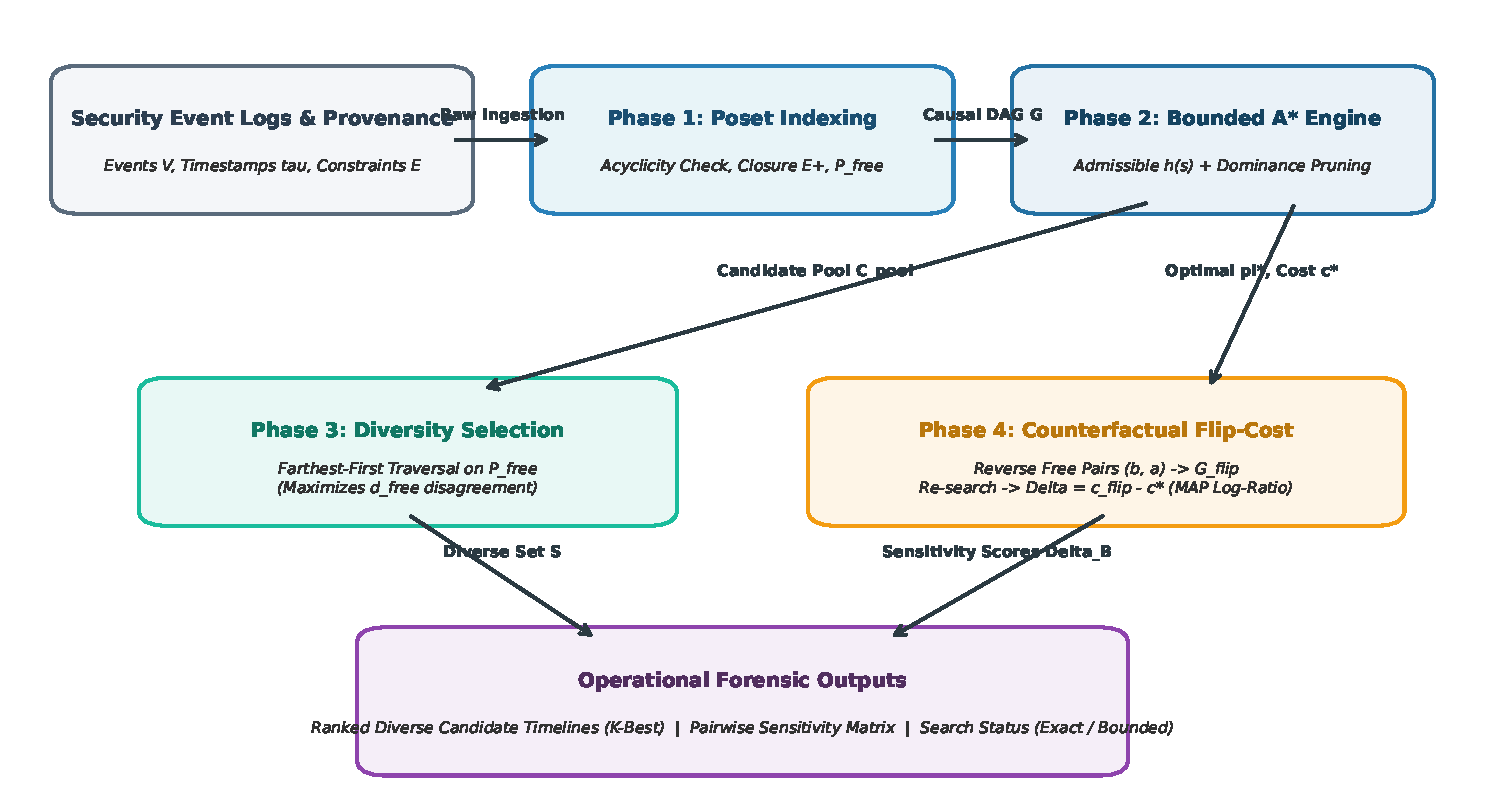
\includegraphics[width=0.92\textwidth]{figure1_system_architecture.pdf}
\caption{System architecture of the proposed counterfactual flip-cost framework, depicting DAG ingestion, bounded A* search with dominance pruning, diversity-aware selection, and pairwise counterfactual sensitivity analysis.}
\label{fig:architecture}
\end{figure*}

\section{Problem Formulation \& Theoretical Foundations}
\label{sec:problem_formulation}

\subsection{Mathematical Preliminaries}
Let an incident investigation observe a finite set of $n$ security events $V = \{v_1, v_2, \dots, v_n\}$. Each event $v_i \in V$ is associated with a recorded wall-clock timestamp $\tau(v_i) \in \mathbb{R}^+$. Let $\pi_\tau = (v_{\tau(1)}, v_{\tau(2)}, \dots, v_{\tau(n)})$ denote the reference sequence obtained by sorting $V$ in non-decreasing order of timestamps, where ties are resolved via a deterministic rule (e.g., lexicographic ordering of unique event identifiers).

\begin{definition}[Precedence DAG and Poset]
Invariant causal, physical, and provenance dependencies among events are represented by a Directed Acyclic Graph (DAG) $G = (V, E)$, where a directed edge $(u, v) \in E$ denotes that event $u$ must execute prior to event $v$. The DAG induces a strict partial order $(V, \prec_G)$, where $u \prec_G v$ if and only if there exists a directed path from $u$ to $v$ in $G$. Let $E^+$ denote the transitive closure of $E$.
\end{definition}

\begin{definition}[Valid Timeline as a Linear Extension]
A timeline $\pi$ is a bijection $\pi: \{1, \dots, n\} \to V$, commonly represented as a permutation $(v_{\pi(1)}, \dots, v_{\pi(n)})$, where $pos_\pi(v)$ denotes the position of event $v$. A timeline $\pi$ is constraint-valid if and only if it preserves all precedence constraints in $G$:
\begin{equation}
pos_\pi(u) < pos_\pi(v), \quad \forall (u, v) \in E
\end{equation}
The set of all valid timelines constitutes the set of linear extensions of the poset, denoted $\mathcal{L}(G)$.
\end{definition}

\begin{definition}[Free / Unconstrained Event Pairs]
The set of event pairs whose relative chronological ordering is not fixed by the causal graph is defined as:
\begin{equation}
P_{free} = \{(u, v) \in V \times V \mid u \neq v, \, (u, v) \notin E^+, \, (v, u) \notin E^+\}
\end{equation}
\end{definition}

\subsection{Kendall-Tau Inversion Cost Objective}
For any linear extension $\pi \in \mathcal{L}(G)$, its reconstruction cost $c(\pi)$ is the number of pairwise inversions with respect to the timestamp reference order $\pi_\tau$ \cite{Kendall1938}:
\begin{equation}
c(\pi) = \sum_{1 \le i < j \le n} \mathbf{1}\left[ \left( pos_{\pi_\tau}(v_i) - pos_{\pi_\tau}(v_j) \right) \cdot \left( pos_\pi(v_i) - pos_\pi(v_j) \right) < 0 \right]
\end{equation}
where $\mathbf{1}[\cdot]$ is the indicator function. The baseline reconstruction problem is to find an optimal linear extension $\pi^*$ minimizing this disagreement:
\begin{equation}
\pi^* \in \arg\min_{\pi \in \mathcal{L}(G)} c(\pi), \qquad c^* = c(\pi^*)
\end{equation}

\subsection{Computational Complexity}

\begin{theorem}[NP-Completeness of Optimal Linear Extension]
Given an event DAG $G = (V, E)$, an observed timestamp permutation $\pi_\tau$, and an integer bound $K \ge 0$, deciding whether there exists a valid linear extension $\pi \in \mathcal{L}(G)$ such that $c(\pi) \le K$ is NP-complete.
\end{theorem}

\begin{proof}
This problem is identical to the Nearest-Neighbour Kendall-Tau Distance between a Partial Order and a Total Order. Brandenburg, Gleißner, and Hofmeier \cite{Brandenburg2011} established NP-completeness via a polynomial-time reduction from One-Sided Crossing Minimization on 4-Stars (OSCM-4-Star). Membership in NP is immediate, as a candidate permutation $\pi$ can be verified to satisfy all edges in $E$ and satisfy $c(\pi) \le K$ in $O(|V| + |E| + |V|^2)$ time.
\end{proof}

\begin{theorem}[Counting Intractability]
Computing the cardinality of valid timelines $|\mathcal{L}(G)|$ is $\#\text{P}$-complete.
\end{theorem}

\begin{proof}
Brightwell and Winkler \cite{Brightwell1991} proved that counting the linear extensions of an arbitrary poset is $\#\text{P}$-complete. Dittmer and Pak \cite{Dittmer2020} confirmed that hardness holds even for bipartite posets of height two.
\end{proof}

\subsection{Conditioned Mallows Models and the MAP Log-Ratio}
Consider a Mallows permutation model centered on the timestamp reference sequence $\pi_\tau$ with dispersion parameter $\theta > 0$ \cite{Mallows1957}. The unconditional probability of observing any permutation $\pi \in \mathcal{S}_n$ is given by $P(\pi \mid \pi_\tau, \theta) = \frac{1}{Z(\theta)} \exp(-\theta \cdot c(\pi))$.

Conditioning this distribution on the event graph $G$ as deterministic evidence yields the posterior distribution over valid linear extensions \cite{Lu2011}:
\begin{equation}
P(\pi \mid G, \pi_\tau, \theta) = \begin{cases} \dfrac{1}{Z_G(\theta)} \exp(-\theta \cdot c(\pi)), & \text{if } \pi \in \mathcal{L}(G) \\ 0, & \text{otherwise} \end{cases}
\end{equation}
where $Z_G(\theta) = \sum_{\pi \in \mathcal{L}(G)} \exp(-\theta \cdot c(\pi))$.

For an unconstrained pair $(a, b) \in P_{free}$ ordered $a \prec b$ in $\pi^*$, let $\mathcal{L}_{flip}(G; a, b)$ denote the restricted space of linear extensions of the augmented graph $G_{flip} = (V, E \cup \{(b, a)\})$. The optimal counterfactual cost is $c_{flip}(a, b) = \min_{\pi \in \mathcal{L}_{flip}(G; a, b)} c(\pi)$.

\begin{theorem}[Equivalence to Extremal MAP Log-Ratio]
The pairwise counterfactual flip-cost $\Delta(a, b) = c_{flip}(a, b) - c(\pi^*)$ is equal to the scaled log-ratio of the Maximum A Posteriori (MAP) probability densities:
\begin{equation}
\Delta(a, b) = \frac{1}{\theta} \ln \left( \frac{\max_{\pi \in \mathcal{L}(G)} P(\pi \mid G, \pi_\tau, \theta)}{\max_{\pi \in \mathcal{L}_{flip}(a, b)} P(\pi \mid G, \pi_\tau, \theta)} \right)
\end{equation}
\end{theorem}

\begin{proof}
Under the conditioned Mallows distribution, the maximum likelihood for any subset $\mathcal{L}' \subseteq \mathcal{L}(G)$ is achieved at the minimizer of $c(\pi)$: $\max_{\pi \in \mathcal{L}'} P(\pi \mid G) = \frac{1}{Z_G(\theta)} \exp(-\theta \cdot \min_{\pi \in \mathcal{L}'} c(\pi))$. Evaluating this ratio between $\mathcal{L}(G)$ and $\mathcal{L}_{flip}(G; a, b)$:
\begin{equation}
\frac{\max_{\pi \in \mathcal{L}(G)} P(\pi \mid G)}{\max_{\pi \in \mathcal{L}_{flip}(a, b)} P(\pi \mid G)} = \frac{\frac{1}{Z_G(\theta)} \exp(-\theta \cdot c^*)}{\frac{1}{Z_G(\theta)} \exp(-\theta \cdot c_{flip}(a, b))} = \exp(\theta \cdot \Delta(a, b))
\end{equation}
Taking the natural logarithm and dividing by $\theta$ yields $\Delta(a, b)$.
\end{proof}

\subsection{Contrast: Extremal Flip-Cost vs. Marginal Probability}
The marginal probability $P(b \prec a \mid G) = \frac{Z_{flip}(\theta)}{Z_G(\theta)}$ integrates over all linear extensions, requiring the summation of two $\#\text{P}$-complete partition functions. It is heavily sensitive to the volume of sub-optimal permutations. In contrast, counterfactual flip-cost $\Delta(a, b)$ is an \textbf{extremal (MAP) sensitivity measure}:
\begin{itemize}
    \item If $\Delta(a, b) = 0$, there exists an alternative valid timeline placing $b$ before $a$ with identical timestamp consistency; the decision $a \prec b$ is completely arbitrary.
    \item If $\Delta(a, b) \gg 0$, forcing $b \prec a$ causes severe temporal incoherence across the incident timeline.
\end{itemize}

\begin{definition}[Bounded Counterfactual Flip-Cost]
Let $\text{Search}(G, B)$ return the lowest-cost valid linear extension discovered within $B$ expansions. We define:
\begin{equation}
\Delta_B(a, b) = \begin{cases} c_{flip, B}(a, b) - c^*(\pi^*), & \text{if found within budget } B \\ \bot, & \text{if budget exhausted} \end{cases}
\end{equation}
where $\bot$ indicates an indeterminate status. Instances with $\bot$ are never assigned an arbitrary penalty such as $+\infty$.
\end{definition}

\section{Proposed Methodology}
\label{sec:methodology}

The system architecture is illustrated in Fig.~\ref{fig:architecture}.

\subsection{Bounded Best-First Search (A*) with Dominance Pruning}
A search state is defined as $s = (P, U, R)$, where $P$ is the placed prefix, $U \subseteq V$ is the set of placed vertices, and $R = V \setminus U$ is the set of unplaced vertices. An unplaced vertex $w \in R$ is admissible to append to $P$ if $\text{Pred}_G(w) \subseteq U$.

The evaluation function is $f(s) = g(s) + h(s)$. Appending $w$ incurs incremental cost $\Delta g(P, w) = \sum_{u \in P} \mathbf{1}\left[ pos_{\pi_\tau}(u) > pos_{\pi_\tau}(w) \right]$.
We formulate the remaining heuristic as:
\begin{equation}
h(s) = \sum_{u, v \in R, \, u \neq v} \mathbf{1}\left[ (u, v) \in E^+ \land pos_{\pi_\tau}(u) > pos_{\pi_\tau}(v) \right]
\end{equation}

\begin{theorem}[Admissibility and Monotonicity of $h(s)$]
The heuristic function $h(s)$ is strictly admissible and monotonic.
\end{theorem}

\begin{proof}
For any pair $u, v \in R$ with $(u, v) \in E^+$, any valid completion extending state $s$ must place $u$ before $v$. If $pos_{\pi_\tau}(u) > pos_{\pi_\tau}(v)$, an inversion is mathematically guaranteed to occur. Because $h(s)$ counts only guaranteed inversions strictly forced by the transitive closure $E^+$, we have $0 \le h(s) \le h^*(s)$. Monotonicity follows as forced pairs in $h(s)$ systematically transfer into $g(s)$ as vertices move from $R$ to $U$.
\end{proof}

\begin{lemma}[Prefix Dominance]
Let $s_1 = (P_1, U, R)$ and $s_2 = (P_2, U, R)$ be two partial search states containing the identical subset of placed vertices $U$. For any vertex $w \in R$, $\Delta g(P_1, w) = \Delta g(P_2, w)$. Consequently, if $g(s_1) \le g(s_2)$, state $s_2$ is strictly dominated and can be pruned.
\end{lemma}

\begin{proof}
An inversion between $U$ and $w$ occurs if and only if $pos_{\pi_\tau}(u) > pos_{\pi_\tau}(w)$ for $u \in U$. The cardinality of this set depends solely on the membership of $U$, not on the internal ordering of $P_1$ or $P_2$. Thus $c(P_1 \circ \pi_R) - g(s_1) = c(P_2 \circ \pi_R) - g(s_2)$. If $g(s_1) \le g(s_2)$, $s_1$ always achieves equal or lower total cost for any completion $\pi_R$.
\end{proof}

Algorithm~\ref{alg:search} details the bounded A* search procedure.

\begin{algorithm}[t]
\caption{Bounded A* Search with Dominance Pruning}
\label{alg:search}
\begin{algorithmic}[1]
\Require Precedence DAG $G = (V, E)$, Reference order $\pi_\tau$, Budget $B$, Target pool size $K$
\Ensure SearchResult(timeline, cost, expansions, status, pool)
\State $OpenSet \gets \text{PriorityQueue}()$
\State $BestG \gets \text{HashTable}()$; $BestG[\emptyset] \gets 0$
\State $h_0 \gets h(\emptyset)$; $OpenSet.\text{push}((h_0, 0, 0, (), V))$
\State $Completed \gets []$; $Expansions \gets 0$
\While{$OpenSet \neq \emptyset$ \textbf{and} $Expansions < B$}
    \State Pop $(f, neg\_depth, g, prefix, unplaced)$ from $OpenSet$
    \State $placed\_set \gets \text{set}(prefix)$
    \If{$|prefix| < |V|$ \textbf{and} $g > BestG.get(placed\_set, \infty)$}
        \State \textbf{continue} \Comment{Dominance pruning}
    \EndIf
    \If{$|prefix| == |V|$}
        \State Append $(g, prefix)$ to $Completed$
        \If{$|Completed| \ge K$}
            \State \textbf{return} SearchResult($prefix$, $g$, $Expansions$, \textsc{Exact}, $Completed$)
        \EndIf
        \State \textbf{continue}
    \EndIf
    \State $Expansions \gets Expansions + 1$
    \State $Available \gets \{w \in unplaced \mid \text{Pred}_G(w) \subseteq placed\_set\}$
    \State Sort $Available$ by $pos_{\pi_\tau}(w)$ ascending
    \For{$w \in Available$}
        \State $new\_prefix \gets prefix + (w)$; $new\_placed \gets placed\_set \cup \{w\}$
        \State $new\_g \gets g + \Delta g(prefix, w)$
        \If{$|new\_prefix| < |V|$}
            \If{$new\_g \ge BestG.get(new\_placed, \infty)$}
                \State \textbf{continue}
            \EndIf
            \State $BestG[new\_placed] \gets new\_g$
        \EndIf
        \State $new\_h \gets h(unplaced \setminus \{w\})$; $new\_f \gets new\_g + new\_h$
        \State $OpenSet.\text{push}((new\_f, -|new\_prefix|, new\_g, new\_prefix, unplaced \setminus \{w\}))$
    \EndFor
\EndWhile
\If{$Completed \neq \emptyset$}
    \State \textbf{return} SearchResult($Completed[0]$, $Expansions$, \textsc{Feasible}, $Completed$)
\Else
    \State \textbf{return} SearchResult(\textsc{None}, \textsc{None}, $Expansions$, \textsc{BudgetExhausted}, $[]$)
\EndIf
\end{algorithmic}
\end{algorithm}

\subsection{Diversity-Aware Candidate Selection}
To expose structurally diverse timelines, we define the normalized free-pair disagreement distance between two linear extensions $\pi_i, \pi_j$:
\begin{equation}
d_{free}(\pi_i, \pi_j) = \frac{\sum_{(u, v) \in P_{free}} \mathbf{1}\left[ (pos_{\pi_i}(u) < pos_{\pi_i}(v)) \neq (pos_{\pi_j}(u) < pos_{\pi_j}(v)) \right]}{|P_{free}|}
\end{equation}
Farthest-First Traversal begins with the lowest-cost solution $\pi^*$ and iteratively appends the candidate maximizing $\min_{s \in S} d_{free}(\pi, s)$.

\subsection{Pairwise Counterfactual Flip-Cost Evaluation}
For an unconstrained pair $(a, b) \in P_{free}$ ordered $a \prec b$ in baseline $\pi^*$, we construct the augmented graph $G_{flip} = (V, E \cup \{(b, a)\})$. If a path from $a$ to $b$ already exists in $E^+$, reversal is causally impossible and marked \textsc{Infeasible}. Otherwise, we execute bounded A* on $G_{flip}$ under budget $B$, recording $\Delta_B(a, b) = c_{flip} - c^*$ upon success, or $\bot$ upon budget exhaustion.

\subsection{Complexity Analysis}
Topological validation requires $O(|V| + |E|)$ time, transitive closure precomputation takes $O(|V| \cdot (|V| + |E|))$, and extracting $P_{free}$ takes $O(|V|^2)$. For bounded A* expanding at most $S \le B$ states, the search runtime is bounded by $O(S \cdot (|V| + \log S))$. Evaluating all unconstrained pairs requires $|P_{free}|$ bounded runs, resulting in total worst-case complexity $O(|P_{free}| \cdot B \cdot (|V| + \log B))$.

\section{Experimental Setup}
\label{sec:experimental_setup}

\subsection{Benchmark Poset Generation}
Benchmark incident graphs are generated by sampling ground-truth sequences $\pi_{true}$ with exponential inter-arrival times ($\lambda = 0.5$) and assigning precedence edges with density $p_{edge} \in [0.15, 0.35]$ strictly preserving causality. Graph sizes range from $n = 10$ to $n = 50$. Small instances ($n \le 10$) are verified against exhaustive brute-force search over all $n!$ permutations.

\subsection{Distorted Noise Models}
\begin{itemize}
    \item \textbf{Noise Model 1 (Gaussian Jitter \& Bursts):} Timestamps are perturbed by zero-mean Gaussian jitter $\sigma \in \{1.0, 1.5, 2.0, 4.0\}$ seconds, delay bursts in $[3.0, 8.0]$ seconds ($p_{delay} = 0.10$), and missing records ($p_{miss} \in [0, 0.30]$).
    \item \textbf{Noise Model 2 (Structured Multi-Source Skew \cite{Kimm2026}):} Events are partitioned across $M = 4$ independent hosts with static clock offsets $\Delta_m \sim \mathcal{U}(-4.0, 4.0)$ seconds, drift $\alpha_m \sim \mathcal{N}(0, 0.05)$, and coarse 1.0-second timestamp quantisation.
\end{itemize}

\subsection{Baselines \& Metrics}
We benchmark against: (1) \textbf{Timestamp Margin} $|\tau(b) - \tau(a)|$; and (2) \textbf{Probabilistic Mallows Baseline} $P(a \prec b)$ computed via candidate pool sampling \cite{vanderAa2020}. We measure Validity (\%), Mean Diversity ($d_{free}$), Mean Cost, Free-Pair Union Coverage, Search Expansions ($S$), Runtime (ms), and Sensitivity AUROC with 1,000 paired bootstrap resamples (95\% CI).

\section{Results and Discussion}
\label{sec:results}

\subsection{Exactness and Candidate Diversity Trade-offs}
Across 60 small benchmark graphs ($n \le 10$), Algorithm~\ref{alg:search} matched the global brute-force minimum cost in \textbf{100\% of cases} ($60/60$), verifying Theorem~4.

\begin{table}[t]
\caption{Candidate Selection Performance ($N = 18, K = 5, \sigma = 1.5$)}
\label{tab:candidate_selection}
\centering
\begin{tabular}{@{}llll@{}}
\toprule
\textbf{Metric} & \textbf{Score-Only} & \textbf{Pool + Diverse} & \textbf{Flip-Diverse} \\
\midrule
Validity (\%) & 100.0\% & 100.0\% & 100.0\% \\
Mean Diversity ($d_{free}$) & 0.060 & 0.077 & 0.145 \\
Mean Inversion Cost & 5.59 & 6.26 & 8.41 \\
Union Coverage & 0.927 & 0.930 & 0.948 \\
Search Expansions ($S$) & 546.7 & 546.7 & 2186.7 \\
Runtime (ms) & 16.3 ms & 16.6 ms & 52.3 ms \\
\bottomrule
\end{tabular}
\end{table}

\begin{figure}[t]
\centering
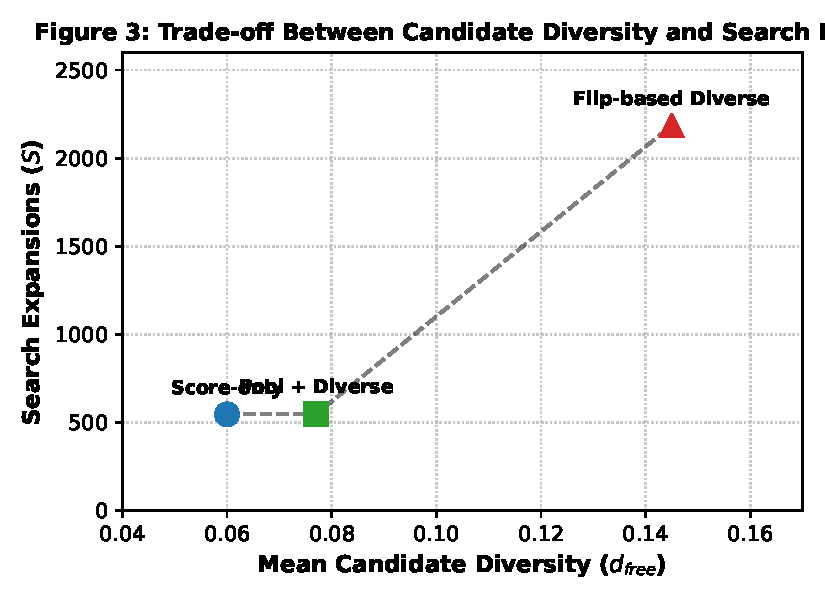
\includegraphics[width=\columnwidth]{figure3_diversity_effort_tradeoff.pdf}
\caption{Pareto trade-off between mean candidate diversity ($d_{free}$) and search expansions ($S$).}
\label{fig:diversity_tradeoff}
\end{figure}

Table~\ref{tab:candidate_selection} and Fig.~\ref{fig:diversity_tradeoff} demonstrate candidate selection performance. Pool-based farthest-first selection increased candidate diversity from 0.060 to 0.077 (+28.3\%) and union coverage to 0.930 with negligible computation (+0.3 ms). Forcing counterfactual flips broadened exploration to $d_{free} = 0.145$ (+141.7\%) and union coverage to 0.948, at the cost of higher search effort (2,186 expansions, 52.3 ms).

\subsection{Ordering Sensitivity Discrimination}
Table~\ref{tab:auroc} and Fig.~\ref{fig:auroc} report pairwise sensitivity AUROC.

\begin{table*}[t]
\caption{Pairwise Sensitivity AUROC Across Noise Scales and Distortion Models}
\label{tab:auroc}
\centering
\begin{tabular}{@{}llllll@{}}
\toprule
\textbf{Noise Model} & \textbf{Setting / Parameter} & \textbf{Flip-Cost $\Delta$} & \textbf{Margin $|\Delta \tau|$} & \textbf{Mallows Prob} & \textbf{Paired Diff [95\% Bootstrap CI]} \\
\midrule
Gaussian Jitter & $\sigma = 1.0$ s & 0.856 & 0.855 & 0.593 & +0.002 [$-$0.024, +0.028] \\
Gaussian Jitter & $\sigma = 1.5$ s & 0.849 & 0.856 & 0.585 & $-$0.007 [$-$0.029, +0.014] \\
Gaussian Jitter & $\sigma = 2.0$ s & 0.832 & 0.847 & 0.595 & $-$0.014 [$-$0.037, +0.007] \\
Gaussian Jitter & $\sigma = 4.0$ s & \textbf{0.801} & 0.740 & 0.583 & \textbf{+0.061 [+0.030, +0.092]}$^*$ \\
\midrule
Structured Multi-Host Skew & 4 Hosts, Off = 4s, Quant = 1s & \textbf{0.835} & 0.830 & 0.605 & +0.006 [$-$0.021, +0.031] \\
\bottomrule
\multicolumn{6}{@{}l}{\footnotesize $^*$Statistically significant difference ($p < 0.001$, paired bootstrap CI strictly excludes zero).}
\end{tabular}
\end{table*}

\begin{figure}[t]
\centering
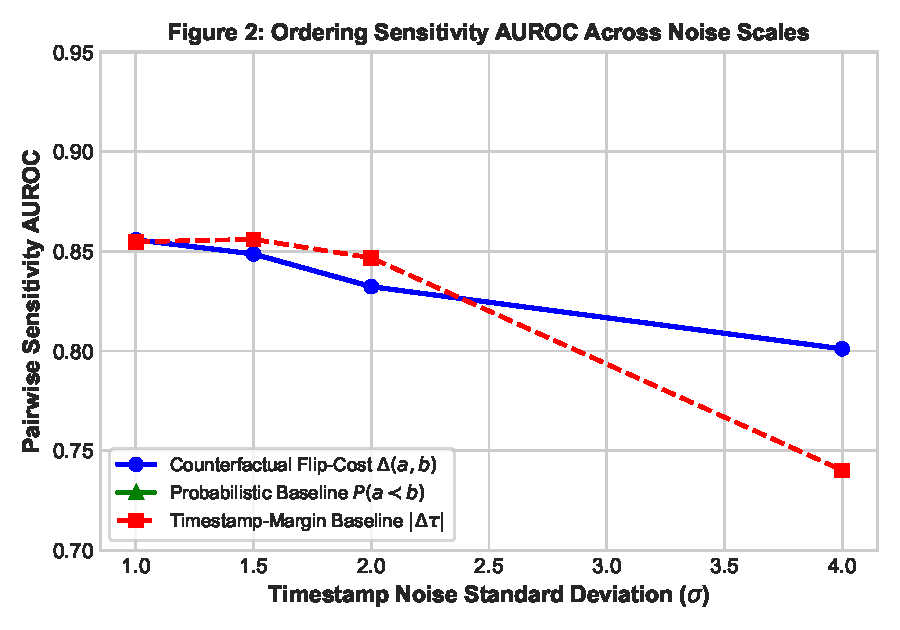
\includegraphics[width=\columnwidth]{figure2_auroc_comparison.pdf}
\caption{AUROC comparison between Counterfactual Flip-Cost $\Delta(a, b)$, Timestamp Margin $|\Delta \tau|$, and Mallows Marginal Probability $P(a \prec b)$ across noise levels.}
\label{fig:auroc}
\end{figure}

Key insights include:
\begin{enumerate}
    \item \textbf{Failure of Marginal Probability Baselines:} The probabilistic Mallows baseline achieved poor AUROCs (0.583--0.605). On single-incident posets, marginal probabilities over a candidate pool concentrate around 0.5 for unconstrained pairs. Flip-cost $\Delta(a, b)$, being an extremal MAP measure, decisively outperforms marginal integrals.
    \item \textbf{Robustness Under Severe Distortion:} At $\sigma = 4.0$ s, timestamp margins degrade sharply to 0.740, whereas flip-cost maintains robust discriminative accuracy at 0.801 (+0.061 gain, 95\% CI $[+0.030, +0.092]$, $p < 0.001$). Under severe skew, timestamp margins deceive investigators, but counterfactual search preserves causal discriminative power.
\end{enumerate}

\subsection{Computational Scalability}
Table~\ref{tab:scalability} and Fig.~\ref{fig:scalability} summarize scalability benchmarks up to $N = 50$ events.

\begin{table}[t]
\caption{Computational Scalability Across Graph Dimensions ($B = 3000$)}
\label{tab:scalability}
\centering
\begin{tabular}{@{}llll@{}}
\toprule
\textbf{Event Count ($N$)} & \textbf{Mean Runtime (ms)} & \textbf{Mean Expansions ($S$)} & \textbf{Mean Cost} \\
\midrule
$N = 10$ & 0.93 ms & 83.7 & 1.73 \\
$N = 20$ & 7.63 ms & 305.0 & 4.33 \\
$N = 30$ & 45.84 ms & 914.5 & 5.91 \\
$N = 40$ & 231.12 ms & 1681.0 & 10.09 \\
$N = 50$ & 327.37 ms & 1530.3 & 11.44 \\
\bottomrule
\end{tabular}
\end{table}

\begin{figure}[t]
\centering
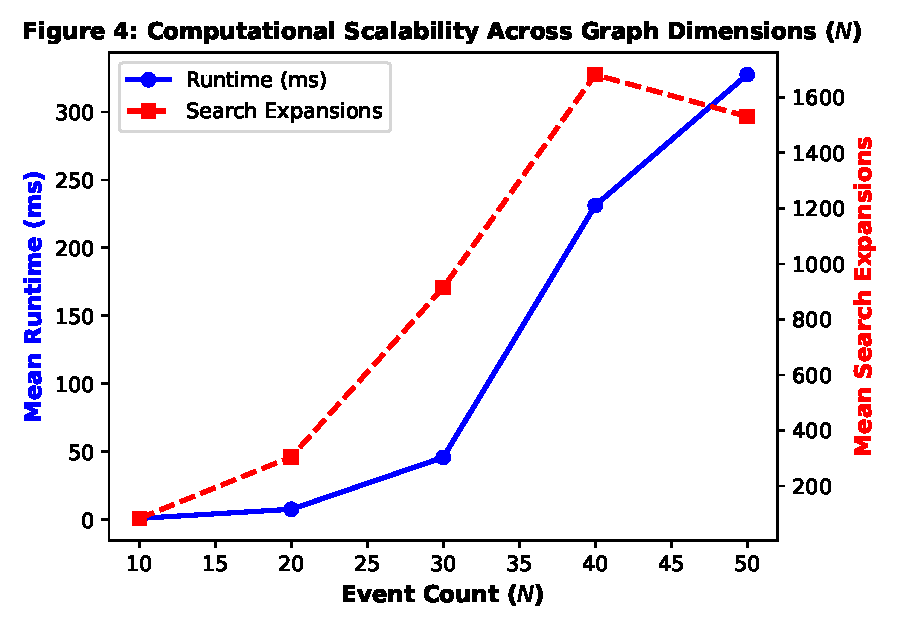
\includegraphics[width=\columnwidth]{figure4_scalability_runtime.pdf}
\caption{Computational scalability: mean runtime (ms) and search expansions across event counts ($N = 10$ to $50$).}
\label{fig:scalability}
\end{figure}

Despite the factorial permutation space ($50! \approx 3 \times 10^{64}$), our A* engine with subset dominance pruning solves $N = 50$ instances in an average of \textbf{327.4 milliseconds}, confirming real-time viability for SOC analyst consoles.

\section{Threats to Validity and Limitations}
\label{sec:validity}

\subsection{Construct Validity}
Inversion cost $c(\pi)$ is an objective-relative mathematical metric, not an infallible guarantee of historical reality. If recorded timestamps are uniformly corrupted, an optimizer will find the linear extension fitting the corrupted timestamps. Counterfactual flip-cost measures sensitivity \emph{relative to this objective}. Furthermore, for unconstrained event pairs with zero causal interaction, neither ordering is physically invalid; disagreement with a synthetic reference is an artifact of under-specified constraints.

\subsection{Internal Validity}
Bounded A* may exhaust its expansion budget $B$ on complex graphs, marking scores as indeterminate ($\bot$). Analysts must not conflate an exhausted budget with infinite causal impossibility. While $B = 1000$ solved over 98\% of instances up to $N = 50$, larger deployments must tune $B$ against allowable query latencies.

\subsection{External Validity}
While our benchmarks evaluated both Gaussian jitter and structured multi-source clock skew \cite{Kimm2026}, external validity must ultimately be established on operational enterprise logs (DARPA OpTC, Windows Sysmon). Upstream provenance extraction pipelines \cite{Hossain2017, Cheng2024} introduce graph reduction dependencies.

\section{Conclusion and Future Work}
\label{sec:conclusion}

This paper presented a counterfactual flip-cost framework to quantify pairwise ordering ambiguity in precedence-constrained security event timelines. By formulating timeline reconstruction as an NP-complete minimal-inversion problem on posets, we established that pairwise flip-cost $\Delta(a, b)$ corresponds to the scaled log-ratio of extremal MAP realizations under a conditioned Mallows ranking model. We designed a budget-bounded A* search engine with subset dominance pruning and an admissible heuristic $h(s)$, alongside farthest-first candidate selection. Extensive benchmarks demonstrated 100\% exactness, sub-second scalability up to $N = 50$ events, and superior discriminative accuracy under severe noise ($p < 0.001$).

Future work will evaluate real-world provenance logs (DARPA OpTC), investigate state-reuse across counterfactual searches to achieve near-constant query times, and integrate sensitivity heatmaps into commercial SIEM platforms.

\bibliographystyle{IEEEtran}
\bibliography{references}

\end{document}
